%%%%%%%%%%%%%%%%%%%%%%%%%%%%%%%%%%%%%%%%%%%%%%%%%%%%%%%%%%%%%%%%%%%%%%%%%%%%%%%%%%%
%% Apresentação do TCC                                                            %%
%% Autor: Gabriel Rufino Montenegro                                               %%
%% Orientador: Prof. Lucas Silveira Melo                                          %%
%% Curso: Engenharia Elétrica - UFC                                               %%
%% Duração: 20 minutos                                                            %%
%%%%%%%%%%%%%%%%%%%%%%%%%%%%%%%%%%%%%%%%%%%%%%%%%%%%%%%%%%%%%%%%%%%%%%%%%%%%%%%%%%%
\documentclass{libs/ufc_format}
\input{libs/preamble.tex}
\bibliography{references.bib}

% Título e subtítulo
\title[FPO com ações de controle em JuMP/Julia]{\Large\textbf{Análise comparativa de formulações de Fluxo de Potência Ótimo com ações de controle em JuMP/Julia}}
\subtitle{Uma progressão incremental F0 $\rightarrow$ F5 com validação sobre redes pedagógicas e um \textit{snapshot} do SIN}
\author{Gabriel Rufino Montenegro}
\institute[EE/UFC]{
    \normalsize{\email{gabrielrufino@alu.ufc.br}}
    \newline
    \department{Orientador: Prof.\ Lucas Silveira Melo}
    \newline
    \department{Departamento de Engenharia Elétrica}
    \newline
    \ufc
}
\date{2026}


%%%%%%%%%%%%%%%%%%%%%%%%%%%%%%%%%%%%%%%%%%%%%%%%%%%%%%%%%%%%%%%%%%%%%%%%%%%%%%%%%%
%% Início do Documento                                                          %%
%%%%%%%%%%%%%%%%%%%%%%%%%%%%%%%%%%%%%%%%%%%%%%%%%%%%%%%%%%%%%%%%%%%%%%%%%%%%%%%%%%
\begin{document}
\input{libs/code_style}

%% ---------------------------------------------------------------------------
% Capa
\begin{frame}{}
    \maketitle
\end{frame}

%% ---------------------------------------------------------------------------
% Sumário
\begin{frame}{Sumário}
    \begin{multicols}{2}
        \tableofcontents
    \end{multicols}
\end{frame}

%% ===========================================================================
\section{Motivação e Objetivos}
%% ===========================================================================

%% ---------------------------------------------------------------------------
\begin{frame}{Contexto: operação do Sistema Interligado Nacional}
    \begin{itemize}
        \item Operação do SIN depende de \example{ações de controle} que vão além do FPO acadêmico:
            \begin{itemize}
                \item \textbf{QLIM} -- limites de geração reativa
                \item \textbf{VLIM} -- limites de magnitude de tensão
                \item \textbf{CSCA} -- bancos \textit{shunt} chaveáveis
                \item \textbf{CTAP} -- \textit{taps} de transformadores em carga
                \item \textbf{DERA} -- esquema hierárquico de corte/alívio de carga
            \end{itemize}
        \item Esses controles são parte da prática do \emph{ANAREDE} (CEPEL)~\cite{cepel2023anarede} e do formato PWF.
        \item Implementados via heurísticas e laços iterativos específicos.
    \end{itemize}

    \vspace{0.3cm}
    \simplebox{\textbf{Pergunta:} como reproduzir esses controles em uma ferramenta moderna e \textit{open-source}?}
\end{frame}

%% ---------------------------------------------------------------------------
\begin{frame}{Lacuna metodológica}
    \begin{columns}
        \begin{column}{0.5\textwidth}
            \begin{block}{PowerModels.jl~\cite{coffrin2018powermodels}}
                \begin{itemize}
                    \item Pacote Julia de referência internacional.
                    \item FPO AC + relaxações DC, SOC, SDP.
                    \item \emph{Sem suporte} aos controles ANAREDE.
                \end{itemize}
            \end{block}
        \end{column}
        \begin{column}{0.5\textwidth}
            \begin{alertblock}{ControlPowerFlow.jl~\cite{chavarry2024}}
                \begin{itemize}
                    \item Proposta de implementação modular dos controles.
                    \item Versão pública \emph{incompleta} (parceria com empresa).
                    \item Inviável como referência direta de comparação.
                \end{itemize}
            \end{alertblock}
        \end{column}
    \end{columns}

    \vspace{0.4cm}
    \successbox{\textbf{Estratégia:} construir do zero, em JuMP, formulações que adicionem os controles ANAREDE um a um, comparáveis às referências PowerModels sobre a mesma bateria de casos.}
\end{frame}

%% ---------------------------------------------------------------------------
\begin{frame}{Objetivos}
    \begin{block}{Objetivo geral}
        Construir, validar e comparar uma progressão incremental de formulações de FP AC em \textbf{JuMP/Julia} sobre o \textit{solver} Ipopt, incorporando as ações de controle ANAREDE.
    \end{block}

    \begin{exampleblock}{Objetivos específicos}
        \begin{enumerate}
            \item Documentar a formulação matemática do FP/FPO em coordenadas polares.
            \item Usar \textit{PWF.jl} para leitura de arquivos ANAREDE com estruturas DOPC/DLIN.
            \item Implementar \emph{duas} formulações de referência via PowerModels.
            \item Implementar \emph{quatro} formulações \textit{hand-built} acrescentando QLIM+VLIM, CSCA, CTAP e DERA.
            \item Submeter as seis formulações a uma bateria de \textbf{27 casos}, do 3 barras ao SIN.
        \end{enumerate}
    \end{exampleblock}
\end{frame}

%% ===========================================================================
\section{Fundamentação Teórica}
%% ===========================================================================

%% ---------------------------------------------------------------------------
\begin{frame}{Fluxo de Potência AC}
    \textbf{Balanço de potência ativa e reativa em cada barra} $i \in \mathcal{N}$:
    \begin{equation*}
        \sum_{(i,j) \in \mathcal{B}_i} p_{ij} = \sum_{k \in \mathcal{G}_i} p^g_k - \sum_{l \in \mathcal{L}_i} p^d_l - g^{sh}_i V_i^2
    \end{equation*}
    \begin{equation*}
        \sum_{(i,j) \in \mathcal{B}_i} q_{ij} = \sum_{k \in \mathcal{G}_i} q^g_k - \sum_{l \in \mathcal{L}_i} q^d_l + b^{sh}_i V_i^2
    \end{equation*}

    \vspace{0.2cm}
    \textbf{Tipos clássicos de barra:}
    \begin{itemize}
        \item \example{Slack}: $V$ e $\theta$ fixos (referência);
        \item \example{PV}: $V$ e $p^g$ especificados;
        \item \example{PQ}: $p^g$ e $q^g$ especificados, $V$ e $\theta$ incógnitas.
    \end{itemize}

    \vspace{0.2cm}
    Sistema algébrico \emph{não linear e não convexo} -- resolvido tipicamente por Newton-Raphson~\cite{vonMeier2006powersystems,gloverSarma2012power}.
\end{frame}

%% ---------------------------------------------------------------------------
\begin{frame}{Fluxo de Potência Ótimo e relaxações}
    \textbf{FPO AC canônico:} adicionar custo e restrições aos limites de equipamentos.
    \vspace{-0.1cm}
    \begin{equation*}
        \min_{V,\theta,p^g,q^g} \sum_{k \in \mathcal{G}} c_k(p^g_k) \quad \text{s.a.} \quad \text{balanço + caixas + } |s_{ij}| \le s^{\max}_{ij}
    \end{equation*}

    \textbf{Relaxações principais} \cite{molzahn2019survey}: aproximação \emph{DC} (LP), relaxação \emph{SOC} (cone), relaxação \emph{SDP} (semidefinida).

    \vspace{-0.15cm}
    \begin{figure}
        \centering
        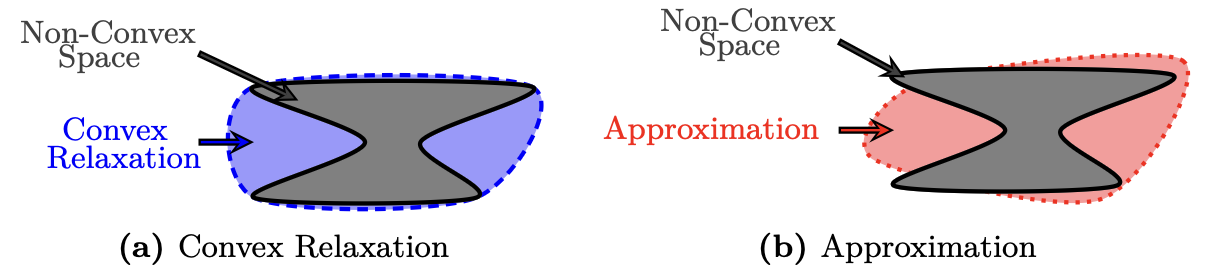
\includegraphics[width=0.68\textwidth]{relaxacao_aproximacao.png}
    \end{figure}
    \vspace{-0.3cm}

    \begin{block}{Comparação no \texttt{case5.m} (\texttt{CodeComparing.jl})}
        \centering
        \begin{tabular}{lcc}
            \hline
            \textbf{Formulação} & \textbf{Característica} & \textbf{Objetivo (US\$/h)} \\
            \hline
            AC-OPF  & Exata, não convexa  & 18\,269{,}10 \\
            DC-OPF  & Aproximação linear  & 17\,613{,}22 \\
            SOC-OPF & Relaxação convexa   & \example{15\,051{,}45} \\
            \hline
        \end{tabular}
    \end{block}

    \vspace{0.1cm}
    \alertbox{O objetivo SOC é uma \emph{cota inferior válida} do AC -- \textit{gap} $\approx 18\%$ neste caso.}
\end{frame}

%% ---------------------------------------------------------------------------
\begin{frame}{Ações de controle do ANAREDE}
    \begin{columns}
        \begin{column}{0.5\textwidth}
            \begin{block}{QLIM + VLIM}
                Lógica de \emph{type-switching} PV $\leftrightarrow$ PQ. Implementada por \example{folgas penalizadas} $s^v_i, s^q_l$ no objetivo.
            \end{block}
            \begin{block}{CSCA}
                Banco \textit{shunt} chaveado $\rightarrow$ $b^{sh}_s \in [b^{sh,\min}, b^{sh,\max}]$ como \emph{variável contínua de decisão}.
            \end{block}
        \end{column}
        \begin{column}{0.5\textwidth}
            \begin{block}{CTAP}
                \textit{Tap} OLTC $\rightarrow$ razão $t_{ij}$ vira \emph{variável contínua}; reaproveita as folgas de tensão de F3 (não cria folga nova).
            \end{block}
            \begin{block}{DERA}
                Corte hierárquico de carga: $\Delta p^d_l \in [0, p^d_l]$ por barra, penalizado por \emph{nível de tensão} (cortar primeiro onde é mais fácil religar).
            \end{block}
        \end{column}
    \end{columns}

    \vspace{0.3cm}
    \simplebox{Todos os controles são introduzidos via \textbf{\textit{soft-constraint}}, evitando o caráter descontínuo dos laços iterativos do ANAREDE.}
\end{frame}

%% ===========================================================================
\section{Metodologia}
%% ===========================================================================

%% ---------------------------------------------------------------------------
\begin{frame}{Pipeline de execução}
    \begin{exampleblock}{Ambiente Julia~\cite{bezanson2017julia}}
        \texttt{PWF.jl}~\cite{pwfjl} (parser ANAREDE) $+$ \texttt{PowerModels.jl}~\cite{coffrin2018powermodels} (referência) $+$ \texttt{JuMP.jl}~\cite{lubin2023jump} (modelagem) $+$ \texttt{Ipopt.jl}~\cite{wachterBiegler2006ipopt} (\textit{solver} NLP).
    \end{exampleblock}

    \vspace{0.1cm}
    \begin{enumerate}
        \item Leitura PWF com \texttt{add\_control\_data=true} (DOPC/DLIN);
        \item Saneamento: maior componente conexa + barra \textit{slack} única;
        \item Padronização das curvas de custo (\texttt{order=2});
        \item Construção da estrutura de referência (\texttt{build\_ref});
        \item Montagem do modelo JuMP (variáveis, fluxos, restrições);
        \item \texttt{optimize!} com \texttt{max\_iter=3000}, \texttt{tol=1e-5};
        \item Exportação CSV (barras e ramos).
    \end{enumerate}

    \vspace{0.15cm}
    \alertbox{\textbf{HVDC:} injeções fixadas via \texttt{JuMP.fix(...; force=true)} -- condição de contorno do FP AC.}
\end{frame}

%% ---------------------------------------------------------------------------
\begin{frame}{A progressão F0 $\rightarrow$ F5}
    \begin{center}
    \footnotesize
    \begin{tabular}{cllll}
        \hline
        \textbf{Sigla} & \textbf{Motor} & \textbf{Tipo} & \textbf{Acrescenta} \\
        \hline
        \example{F0} & PowerModels & FPO AC          & \textit{baseline} FPO \\
        \example{F1} & PowerModels & FP AC           & \textit{baseline} FP \\
        F2 & JuMP \textit{hand-built} & FP controlado & QLIM + VLIM \\
        F3 & JuMP \textit{hand-built} & FP controlado & + CSCA \\
        F4 & JuMP \textit{hand-built} & FP controlado & + CTAP \\
        F5 & JuMP \textit{hand-built} & FP controlado & + DERA \\
        \hline
    \end{tabular}
    \end{center}

    \vspace{0.3cm}
    \successbox{\textbf{Progressão estritamente aditiva:} cada formulação parte da anterior e acrescenta um único bloco de variáveis e restrições. Qualquer divergência entre dois \textit{scripts} consecutivos é atribuível ao \emph{novo controle introduzido}.}
\end{frame}

%% ---------------------------------------------------------------------------
\begin{frame}{Como funcionam as folgas penalizadas}
    \textbf{Exemplo de F2 (QLIM + VLIM):}

    \begin{itemize}
        \item Variáveis primárias: $V_i, \theta_i, p^g_k, q^g_k$ com limites caixa do PWF.
        \item Folgas: $s^v_i$ em cada barra PV, $s^q_l$ em cada carga.
        \item Restrição de \textit{setpoint}: $V_i = V^{ref}_i + s^v_i$.
        \item Função objetivo \textit{soft-constraint}:
            \begin{equation*}
                \min \; \rho \sum_{i \in \mathcal{N}^{gen}} (s^v_i)^2 + \rho \sum_{l \in \mathcal{L}} (s^q_l)^2, \quad \rho = 10^6
            \end{equation*}
    \end{itemize}

    \vspace{0.3cm}
    \begin{exampleblock}{Intuição}
        Se o problema é factível com $s^v = s^q = 0$, o ótimo respeita os \textit{setpoints}. Caso contrário, viola \emph{minimamente} -- ao invés de declarar \texttt{INFEASIBLE} como o FP clássico.
    \end{exampleblock}
\end{frame}

%% ===========================================================================
\section{Resultados}
%% ===========================================================================

%% ---------------------------------------------------------------------------
\begin{frame}{Bateria de testes -- 27 casos}
    \begin{itemize}
        \item \textbf{Redes pedagógicas (3--9 barras):} \texttt{3bus}, \texttt{3busfrank}, \texttt{4busfrank\_vlim}, \texttt{5busfrank}, \texttt{9bus} e variantes (\texttt{\_DBSH}, \texttt{\_DCER}, \texttt{\_DCSC}, \texttt{\_DCline}, \texttt{\_csca}, \texttt{\_ctap}, \dots).
        \item \textbf{Médio porte:} \texttt{300bus}, \texttt{500bus}.
        \item \textbf{Recortes do SIN-Nordeste (PAR/PEL 2027--2031):} \texttt{caso\_red} (2\,599 barras), \texttt{caso\_red2} (1\,033 barras).
        \item \textbf{\textit{Snapshot} integral do SIN:} \texttt{CASO\_VER\_MAXDIU} (13\,338 barras, PAR/PEL 2027--2031, Verão Máx.\ Diurna).
        \item \textbf{Casos de \textit{stress}:} \texttt{test\_defaults}, \texttt{test\_line\_shunt}, \texttt{test\_system}.
    \end{itemize}

    \vspace{0.3cm}
    \simplebox{Critério de equivalência numérica entre formulações: $|\Delta| \le 10^{-4}$ simultaneamente sobre $V, \theta, p^g, q^g$ e fluxos de ramo.}
\end{frame}

%% ---------------------------------------------------------------------------
\definecolor{statusok}{RGB}{198,239,206}
\definecolor{statusinf}{RGB}{255,235,156}
\definecolor{statuskil}{RGB}{255,199,206}
\definecolor{statusinv}{RGB}{244,176,132}

\begin{frame}{Convergência global -- \emph{hand-built} ganham faixa}
    \footnotesize
    \begin{center}
    \renewcommand{\arraystretch}{1.1}
    \setlength{\tabcolsep}{4pt}
    \begin{tabular}{lcccccc}
        \hline
        \textbf{Caso (resumo)} & \textbf{F0} & \textbf{F1} & \textbf{F2} & \textbf{F3} & \textbf{F4} & \textbf{F5} \\
        \hline
        \texttt{3bus} (padrão)         & \cellcolor{statusok}OK & \cellcolor{statusok}OK & \cellcolor{statusok}OK & \cellcolor{statusok}OK & \cellcolor{statusok}OK & \cellcolor{statusok}OK \\
        \texttt{9bus}                  & \cellcolor{statusok}OK & \cellcolor{statusok}OK & \cellcolor{statusok}OK & \cellcolor{statusok}OK & \cellcolor{statusok}OK & \cellcolor{statusok}OK \\
        \texttt{300bus}                & \cellcolor{statusinv}INV & \cellcolor{statusok}OK & \cellcolor{statusok}OK & \cellcolor{statusok}OK & \cellcolor{statusok}OK & \cellcolor{statusok}OK \\
        \texttt{500bus}                & \cellcolor{statusinf}INF & \cellcolor{statusok}OK & \cellcolor{statusok}OK & \cellcolor{statusok}OK & \cellcolor{statusok}OK & \cellcolor{statusok}OK \\
        \texttt{4busfrank\_vlim}       & \cellcolor{statusinf}INF & \cellcolor{statusinf}INF & \cellcolor{statusok}OK & \cellcolor{statusok}OK & \cellcolor{statusok}OK & \cellcolor{statusok}OK \\
        \texttt{5busfrank\_csca}       & \cellcolor{statusinf}INF & \cellcolor{statusinf}INF & \cellcolor{statusok}OK & \cellcolor{statusok}OK & \cellcolor{statusok}OK & \cellcolor{statusok}OK \\
        \texttt{caso\_red}             & \cellcolor{statusinf}INF & \cellcolor{statusok}OK & \cellcolor{statusok}OK & \cellcolor{statusok}OK & \cellcolor{statusok}OK & \cellcolor{statusok}OK \\
        \texttt{caso\_red2}            & \cellcolor{statusinf}INF & \cellcolor{statusinf}INF & \cellcolor{statusok}OK & \cellcolor{statusok}OK & \cellcolor{statusok}OK & \cellcolor{statusok}OK \\
        \texttt{CASO\_VER\_MAXDIU}      & \cellcolor{statuskil}KIL & \cellcolor{statusinf}INF & \cellcolor{statuskil}KIL & \cellcolor{statusinf}INF & \cellcolor{statuskil}KIL & \cellcolor{statusinf}INF \\
        \hline
    \end{tabular}
    \end{center}

    \vspace{0.2cm}
    \successbox{\textbf{F2--F5 convergem em 23 casos}, vs.\ 18 de F1 e 15 de F0 (bateria completa).}
\end{frame}

%% ---------------------------------------------------------------------------
\begin{frame}{Análise barra a barra -- \textit{clusters} de equivalência}
    \textbf{Exemplo: \texttt{3bus\_DCSC} -- quatro \textit{clusters} distintos.}
    \begin{center}
    \footnotesize
    \begin{tabular}{ccrr}
        \hline
        \textbf{Barra} & \textbf{Formulação} & $V$ (p.u.) & $\theta$ (rad) \\
        \hline
        1 & F0      & 1{,}1000 & 0{,}0000 \\
        1 & F1      & 1{,}0290 & 0{,}0000 \\
        1 & F2      & 1{,}0352 & 0{,}0000 \\
        1 & F3 a F5 & 1{,}0064 & 0{,}0000 \\
        \hline
        3 & F0      & 1{,}0698 & $-1{,}8 \times 10^{-2}$ \\
        3 & F1      & 0{,}9970 & $-2{,}5 \times 10^{-2}$ \\
        3 & F2      & 1{,}0178 & $-1{,}2 \times 10^{-2}$ \\
        3 & F3 a F5 & 0{,}9878 & $-1{,}3 \times 10^{-2}$ \\
        \hline
    \end{tabular}
    \end{center}

    \vspace{0.2cm}
    \begin{itemize}
        \item \example{F0}: FPO empurra $V \to 1{,}1$\,p.u.\ (limite caixa).
        \item \example{F1}: ponto operacional ``natural'' do FP clássico.
        \item \example{F2}: próximo de F1, com folga $s^v$ residual.
        \item \example{F3--F5}: CSCA ajusta $b^{sh}_s$ $\Rightarrow$ tensões mais baixas.
    \end{itemize}
\end{frame}

%% ---------------------------------------------------------------------------
\begin{frame}{Destaque: o \texttt{caso\_red2} (CE+RN+PB, 1\,033 barras)}
    \begin{block}{Sintoma do FP clássico (F1)}
        Declara \texttt{LOCALLY\_INFEASIBLE} em uma solução fisicamente impossível:
        \[ V_{\min} = \emph{$-0{,}431$\,p.u.}, \qquad V_{\max} = \emph{1{,}935\,p.u.} \]
    \end{block}

    \begin{exampleblock}{Resposta das formulações controladas}
        \centering
        \footnotesize
        \begin{tabular}{lcrrr}
            \hline
            \textbf{Formulação} & \textbf{Status} & \textbf{Objetivo} & $V_{\min}$ & $V_{\max}$ \\
            \hline
            F1 (FP-Ref)  & \emph{INF} & 0                                  & $-0{,}431$ & 1{,}935 \\
            F2 (QLIM+VLIM) & OK       & $4{,}94 \times 10^{2}$             & 0{,}950 & 1{,}231 \\
            F3 (+CSCA)     & OK       & $2{,}16 \times 10^{2}$             & 0{,}950 & 1{,}228 \\
            F4 (+CTAP)     & OK       & \example{$9{,}56 \times 10^{-2}$}  & 0{,}950 & 1{,}269 \\
            \hline
        \end{tabular}
    \end{exampleblock}

    \vspace{0.2cm}
    \successbox{\textbf{F4} reduz o objetivo $\sim$\,\emph{5\,000$\times$} em relação a F2: CSCA+CTAP encontra um ponto praticamente compatível com os \textit{setpoints} do PWF.}
\end{frame}

%% ---------------------------------------------------------------------------
\begin{frame}{O caso SIN integral (\texttt{CASO\_VER\_MAXDIU})}
    \begin{alertblock}{Resultado negativo, mas relevante}
        \emph{Nenhuma} das seis formulações converge dentro do orçamento (\texttt{max\_iter=3000}, \textit{wall time}):
        \begin{itemize}
            \item F0, F2, F4 atingem o \textbf{limite de tempo} (KIL);
            \item F1, F3, F5 terminam em \textbf{LOCALLY\_INFEASIBLE}.
        \end{itemize}
    \end{alertblock}

    \vspace{0.2cm}
    \begin{itemize}
        \item As formulações \emph{já partem} do ponto convergido do ANAREDE lido do PWF -- a inicialização \emph{não} é o gargalo.
        \item Causa provável: fidelidade do modelo NLP reconstruído (HVDC, intercâmbios, controles remotos, múltiplas referências) + condicionamento com $\rho = 10^6$ nessa escala.
        \item \example{Boa notícia:} a infraestrutura (leitura PWF, \texttt{build\_ref}, modelo JuMP, chamada Ipopt) funciona corretamente em escala SIN -- não há \texttt{CRA} nem \texttt{ERR}.
        \item Obstáculo é \emph{numérico}, não estrutural.
    \end{itemize}
\end{frame}

%% ---------------------------------------------------------------------------
\begin{frame}{Verificação auxiliar FDC: o mesmo SIN, em DC, converge}
    \begin{exampleblock}{FDC -- fluxo de potência DC (\texttt{solve\_dc\_pf}) sobre \texttt{CASO\_VER\_MAXDIU}}
        Mesmo \textit{pipeline}, mesmo arquivo, mesma máquina: encerra em \example{\texttt{LOCALLY\_SOLVED}} em poucas iterações.
    \end{exampleblock}

    \begin{columns}
        \begin{column}{0.5\textwidth}
            \footnotesize
            \renewcommand{\arraystretch}{1.1}
            \begin{tabular}{lr}
                \hline
                \textbf{Métrica} & \textbf{Valor} \\
                \hline
                Status           & \texttt{LOCALLY\_SOLVED} \\
                Barras retidas   & 13\,283 \\
                Geração ativa    & $\approx$ 70{,}97\,GW \\
                Carga ativa      & $\approx$ 69{,}57\,GW \\
                Perdas (DC)      & 0 (desprezadas) \\
                Ângulos extremos & $-166^\circ$ a $+177^\circ$ \\
                \hline
            \end{tabular}
        \end{column}
        \begin{column}{0.5\textwidth}
            \begin{itemize}
                \item Confirma: o obstáculo do AC é \emph{numérico}, não estrutural.
                \item Mas ângulos de $\pm 170^\circ$ \emph{violam} a hipótese da linearização $\Rightarrow$ a solução DC não é fisicamente realizável.
            \end{itemize}
        \end{column}
    \end{columns}

    \vspace{0.2cm}
    \successbox{O valor da FDC é \emph{diagnóstico}, não de inicialização: com $V = 1{,}0$ e ângulos de $\pm 177^\circ$, a solução DC é ponto de partida \emph{pior} que o próprio ponto convergido do ANAREDE já utilizado -- ela \emph{não} serve de \textit{warm-start}.}
\end{frame}

%% ===========================================================================
\section{Conclusões}
%% ===========================================================================

%% ---------------------------------------------------------------------------
\begin{frame}{Síntese das contribuições}
    \begin{exampleblock}{1. Faixa de convergência ampliada}
        F2--F5 convergem em \emph{23 dos 27 casos}; em 9 casos, encontram solução factível enquanto ao menos uma das referências falha.
    \end{exampleblock}

    \begin{exampleblock}{2. \textit{Fingerprint} computacional dos controles}
        \textit{Clusters} de equivalência reproduzem o efeito esperado de cada controle:
        $\{$F1,F2$\}$ quando folgas saturam em zero; $\{$F3,F4$\}$ em redes com CSCA/CTAP ativo; F5 forma cluster próprio só em redes com margem reativa estreita.
    \end{exampleblock}

    \begin{alertblock}{3. Fronteira numérica atual}
        Nenhuma formulação converge no SIN, mesmo partindo do ponto convergido do ANAREDE e com orçamento de 3\,000 iterações. Delimita com clareza onde a abordagem \textit{soft-constraint} pura precisa de reconciliação de modelo e melhor condicionamento.
    \end{alertblock}
\end{frame}

%% ---------------------------------------------------------------------------
\begin{frame}{Limitações e trabalhos futuros}
    \begin{columns}
        \begin{column}{0.5\textwidth}
            \begin{alertblock}{Limitações}
                \begin{itemize}
                    \item $b^{sh}_s$ (CSCA) e $t_{ij}$ (CTAP) \emph{contínuos}; operação real é discreta.
                    \item DERA: corte de carga contínuo/suave, vs.\ ERAC discreto e emergencial.
                    \item HVDC com fluxos fixados como condição de contorno.
                \end{itemize}
            \end{alertblock}
        \end{column}
        \begin{column}{0.5\textwidth}
            \begin{exampleblock}{Trabalhos futuros}
                \begin{itemize}
                    \item Viabilizar SIN: verificação de resíduos, auditoria da tradução PWF$\to$JuMP e homotopia das penalidades $\rho$.
                    \item Discretizar CSCA/CTAP $\rightarrow$ MINLP (Juniper/Alpine).
                    \item Acoplar F2--F5 ao \textit{ControlPowerFlow.jl} como \textit{oracle} de validação.
                \end{itemize}
            \end{exampleblock}
        \end{column}
    \end{columns}

    \vspace{0.4cm}
    \simplebox{\textbf{Repositório do trabalho:} \texttt{powerflow/Codes/PF\_Formulation/}}
\end{frame}

%% ---------------------------------------------------------------------------
% Referências
\begin{frame}[allowframebreaks]
    \frametitle{Referências}
    \nocite{Template_Beamer_UFC}
    \printbibliography
\end{frame}

%% ---------------------------------------------------------------------------
% Slide de encerramento
\begin{frame}{}
    \centering
    \huge{\textbf{\example{Obrigado pela atenção!}}}

    \vspace{1cm}

    \Large{\textbf{Dúvidas?}}

    \vspace*{0.8cm}
    \normalsize Gabriel Rufino Montenegro \\
    \vspace{0.2cm}
    \large{\email{gabrielrufino@alu.ufc.br}}

    \vspace{0.6cm}
    \footnotesize Orientador: Prof.\ Lucas Silveira Melo
\end{frame}

\end{document}
